
%Performance is a significant factor when evaluating a parallel programming model.  
In this section we compare our task-based implementations to the original \PARSEC{} implementations in Pthreads or OpenMP.

\subsection{Scalability}
\label{subsec:scalability}
Figures~\ref{fig:scalability_graphs_1},\ref{fig:scalability_graphs_2},\ref{fig:scalability_graphs_3},\ref{fig:scalability_graphs_4} 
shows how the task-based codes scale compared to the \PARSEC{} Pthread/OpenMP versions. 
Results are shown individually per benchmark as we increase the number 
of cores assigned to the application and normalized to the execution time of the serial implementation
\footnote{The PARSEC benchmark suite provides a serial implementation for \texttt{blackscholes}, \texttt{bodytrack}, \texttt{dedup}, \texttt{ferret}, 
\texttt{freqmine} and \texttt{swaptions}. 
For the other benchmarks, the original Pthreads parallel implementation executed on a single core is considered as the baseline.}
 of the application. Nearly all applications scale linearly up to 4 cores.
%However, with 8 and 16 cores, 
%performance improvements diminish.
%reaching 30\%, 42\% and 34\% improvements, respectively.

In the case of \texttt{bodytrack}, as described in Section~\ref{sec:parsecss_implementation}, by concurrently executing different frames, there is always enough work for all threads, while by taskifying the 
output stage of each frame, we overlap this I/O bottleneck with other computation stages. The speedup when run on 16 cores is 12.1x, while the Pthreads implementation reaches a poor 6.8x speedup when run on 16 cores.
The \texttt{dedup} application has a very expensive stage that writes the compressed data to the output file. 
Our task-based implementation is very effective in overlapping this time with computation from the compression stage. Also, the task-based version does not have to reorder the data chunks, 
since the I/O execution takes place in-order as dictated by dataflow relations. This results in an impressive 30\% performance improvement of the OmpSs version with respect to Pthreads when run on 16 cores.
The Pthreads \texttt{facesim} implementation is burdened by barriers that limit available parallelism. 
By using dataflow relations 
%among 
%the different parallel loops and stages, we remove all barriers, except the barriers before starting and finishing the \texttt{CG} kernel,
%which protect the residual calculation. In Section~\ref{sec:implementation} we discuss two different 
%implementations, one only with tasks and one using also OpenMP equivalent loops. Figure\ref{fig:scalability_graphs} shows the speedup for the later version.
%Our initial implementation gave 8.7\% performance improvement compared to the Pthreads version. 
%The issue with our initial approach was that
%some tasks had very high task creation overhead, which led to unfavorable scheduling and load imbalance among threads. 
%We identified some opportunities 
%to overlap computation with task creation, hiding any runtime overheads, but this did not eliminate them completely. By using the loop construct 
%we managed to minimize the task creation overhead. 
we taskify sequential segments of significant cost we effectively
synchronize them with parallel sections preceding and following it.
The performance improvements comes from the overlap of sequential computations with parallel sections.
The task-based parallelization of \texttt{facesim} reaches a speedup of 10.2x when run on 16 cores, while the PARSEC code only reaches a 6.4x speedup.

In the cases of \texttt{blackscholes}, \texttt{canneal}, \texttt{ferret}, \texttt{fluidanimate}, \texttt{freqmine} and \texttt{swaptions}, the Pthreads/OpenMP
versions already achieve good scalability results. With the exception of \texttt{ferret}, the task-based codes have very close resemblance to their Pthreads/OpenMP counterparts, and have offered reduced 
opportunities for \OMPSS{} to dynamically exploit additional parallelism.  
The parallel implementation in these applications, with the exception of \texttt{ferret}, is limited to parallel do-all loops with 
barrier synchronization, essentially exploiting the same amount of parallelism among all versions (OmpSs/Pthreads/OpenMP). 

In the case of \texttt{ferret}, although the code is substantially different, both versions employ the same pipeline model and deliver the same level of parallelism, which is already  high in the Pthread version.  
We express 
a bit of extra parallelism by extending the pipeline with multiple stages, which write to the output file, effectively overlapping some communication with computation. 
However, the final impact in the 
total execution time is limited as the time needed to write the output file is a very small fraction of the total execution time. 
Finally, we observe performance gain (18\%) in \texttt{streamcluster}, which can be partly attributed to the more efficient 
barrier implementation of \OMPSS{}, when compared to the user implemented barriers of the Pthreads version. 
However, the most important performance drawback 
that the original Pthreads implementation suffers from, is the negative NUMA effects.
This issue is observed when we run our experiments on a two socket system.
The Pthreads code partitions the working set by the number of available cores.
We employ a different partition scheme to counter the 
NUMA effects. Through experimentation we observe that the best results can be obtained when using 80 blocks. 

%However, when we use the 
%same number of partitions as the Pthreads version, which is 16, we obtain a moderate speedup of 9\%.  We can observe how the 
%same results in figure~\ref{fig:granularity_comparison}.  Green bar represents the task-based version 
%that uses the same granularity as Pthreads, while the blue bar shows the performance of \texttt{streamcluster}, when using 80 blocks.

\begin{figure}[t]
  \centering
  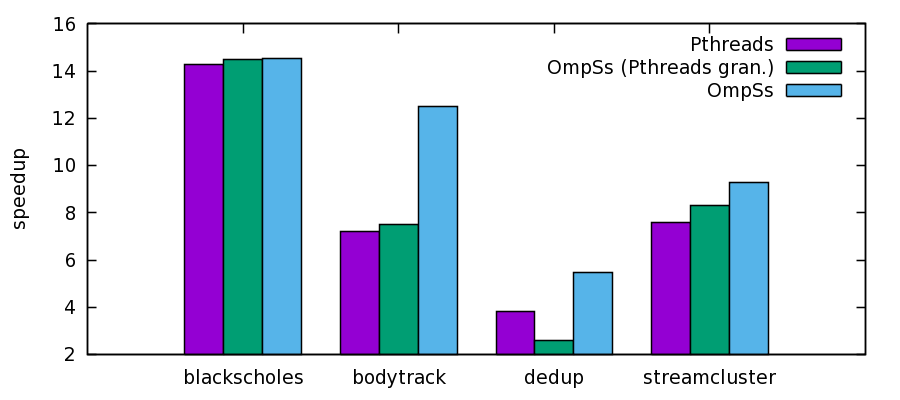
\includegraphics[width=.9\textwidth]{task_benchmarks/figures/parsec_comparison}
  \caption{Speedup comparison for Pthreads and OmpSs with the same granularity, as well as our optimized OmpSs version, when run on 16 cores. Results are normalized to the sequential version of the original code.}
  \label{fig:granularity_comparison}
	\vspace{0.5cm}
\end{figure}

\subsection{Task Granularity Impact}
The granularity of individual tasks is an important factor that needs to be considered when parallelizing an application.
Small task granularity can reduce load imbalance  
but such performance benefits can be neglected by the overhead of the runtime system, as it has to create and schedule more tasks.
Results in Section~\ref{subsec:scalability} show how tuning the task granularity brings performance benefits in some cases (\texttt{blackscholes}, \texttt{bodytrack}, \texttt{dedup} and \texttt{streamcluster})
while in others it is better to keep the same parallel granularity as the \PARSEC{} distribution codes (\texttt{canneal}, \texttt{facesim}, \texttt{ferret}, \texttt{freqmine} and \texttt{swaptions}).
 
In order to provide a more comprehensive comparison, this section examines the performance 
of \texttt{blackscholes}, \texttt{bodytrack}, \texttt{dedup} and \texttt{streamcluster} when using exactly the same granularity as in the \PARSEC{} distribution code.
Figure~\ref{fig:granularity_comparison} shows the speedup of these benchmarks when run on 16 cores. 
The purple bar shows the speedup of the Pthreads version, the green one shows the speedup of a task-based implementation that has the same parallel granularity as its Pthreads counterpart.
Finally, the light blue bar shows the speedup of the optimal task-based implementations discussed in Sections~\ref{sec:parsecss_implementation} and~\ref{subsec:scalability}. 

For the cases of \texttt{blackscholes} and \texttt{streamcluster} the parallelization scheme followed in the three codes (Pthreads and the two OmpSs versions) is the same. 
The difference between the two OmpSs versions is the granularity of the block sizes that are processed per task.
In case of \texttt{blackscholes}, the OmpSs implementation with the same granularity as Pthreads does not perform better since the parallelism of this benchmark follows a fork-join model.
In the case of \texttt{streamcluster}, the task-based implementations always improve the Pthreads performance, even if they operate following the same parallelization scheme and granularity as the Pthreads version.
These improvements come from the NUMA effects correction that the OmpSs versions carry out.

In the case of \texttt{bodytrack} the optimal OmpSs implementation follows a quite different parallelization scheme than the original Pthreads code, as explained in Section~\ref{sec:parsecss_implementation}. 
We consider a trivial implementation in OmpSs where we follow the same parallelization strategy as in Pthreads. 
As shown in Figure~\ref{fig:granularity_comparison}, we do not observe any significant difference in performance among Pthreads and the equivalent OmpSs implementation. 
However, the new parallelization scheme is not applicable to Pthreads as it requires to synchronize the workload by explicit dependencies, which are not available in the Pthreads API.

In the case of \texttt{Dedup}, the trivial Pthreads-like implementation performs poorly, achieving a speedup of 2.6x. 
In this implementation, each pipeline stage is taskified following the Pthreads approach. 
Each large chunk is partitioned into smaller chunks, that will spawn three new tasks (\texttt{Compress}, \texttt{Deduplicate}
and \texttt{WriteOutput}). 
This level of granularity creates hundreds of thousands of tasks, increasing the runtime's overhead significantly. 
In contrast, the optimized task-based version operates at the granularity of the large chunks, creating only a few hundreds of tasks, effectively reducing the runtime overhead. 
%The number of tasks is not the only factor that can influence performance, as their duration is also important. In the fine grain task-based version, some tasks take a very short time to execute. 
%For example \texttt{Deduplication} tasks simply try to insert a single new chunk in a hashtable.

%In general, when following the exact same parallelization strategy and task granularity, Pthreads and OmpSs obtain very similar performance. However, the number of tasks and their size can negatively impact the overall performance. Consequently, users should avoid flooding the runtime system with tasks that run for very short time. Finally, the asynchronous nature of task-based programming models and their programmability allows the users to tune the parallelization strategy or implement more advanced techniques that lead to better final performance.
In some cases, OmpSs can over-perform Pthreads even if the same parallelization scheme and granularity is followed, like the \texttt{streamcluster} results demonstrate.
In some other cases (\texttt{dedup} and \texttt{bodytrack}), the performance improvements come from an optimized parallelization scheme.
Such new schemes could be hardly implemented in Pthreads since they require a direct synchronization via explicit dependencies, which is not available in the Pthreads API.
Finally, in case of simple fork-join applications (i. e. \texttt{blackscholes}) our performance benefits just come from further optimizing the parallel granularity.


\begin{figure*}[p]
  \centering
  \begin{subfigure}{0.75\textwidth}
                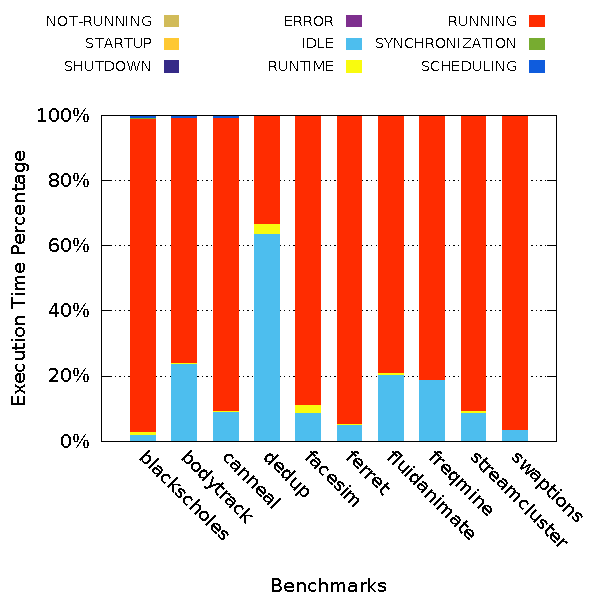
\includegraphics[width=\textwidth]{task_benchmarks/figures/worker-runtime-breakdowns-8}
                \caption{Average time over 8 threads}
                \label{fig:runtime_breakdown_8}
  \end{subfigure}
	\hfill
  \begin{subfigure}{0.75\textwidth}
                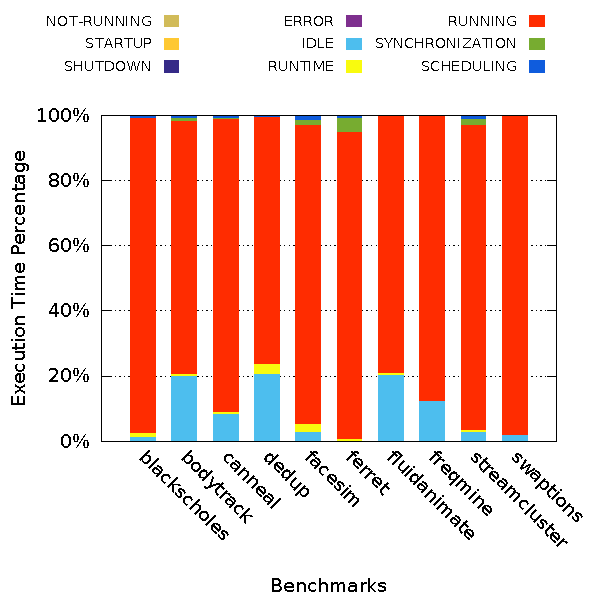
\includegraphics[width=\textwidth]{task_benchmarks/figures/master-runtime-breakdowns-8}
                \caption{Main thread runtime breakdowns}
                \label{fig:master_runtime_breakdown_8}
  \end{subfigure}
        \caption{Runtime breakdowns when running on an 8-core configuration.}
        \label{fig:runtime_breakdown}
	\vspace{.5cm}
\end{figure*}



%\vspace{-0.8cm}
\subsection{Runtime System Overhead}
%\vspace{-0.15cm}
Task creation, scheduling and data dependencies tracking are all handled by the OmpSs runtime system. In this section, we evaluate the impact of these activities over the final parallel performance.
Figure~\ref{fig:runtime_breakdown_8} shows a breakdown of the total execution time of each application. 
Each bar shows the breakdown of one application after averaging the values over eight concurrently executing threads.
The red color represents the portion of time dedicated in running tasks, that is, in running user code. 
All applications, excluding dedup, spend more than 75\% of time doing useful work. 
The cyan bar represents idle time, 
which corresponds to the time a thread is waiting for some work to become available and is caused by load imbalance and sequential code phases. 
In most cases this time is low, except for \texttt{dedup},
where it reaches 60\% of the total execution time. 
In Figure~\ref{fig:runtime_breakdown_8} we also represent the time spent in other activities like synchronization, scheduling, etc. 
None of these activities represent more than 5\% of the total execution time.

Figure~\ref{fig:master_runtime_breakdown_8} shows the same breakdown of execution time but only for the main
thread of execution, which is the one that runs serial parts of the code besides parallel tasks.
\texttt{Dedup} has significantly lower idle time in the main thread, which indicates that there is not enough parallel work to keep all                                                        
threads busy.
This issue has been previously reported~\cite{Vandierendonck:2013:DSP:2503210.2503233}.
In general we see that the overhead of the runtime system is low, with only a few cases that show some time spent in synchronization, scheduling, 
and miscellaneous runtime overhead (in light yellow).
Synchronization time can be time spent waiting a barrier or acquiring/releasing locks. Scheduling includes time needed to resolve dependencies 
and make scheduling decisions, while other runtime overheads are related to activity that cannot be associated with task scheduling and creation.
Overall, we have seen that our implementations improve scalability considerably (by \AVERAGEPERF{} on average), while runtime overhead remains low.

\begin{table*}[!t]
        \centering
        \scriptsize
        \caption{\PARSEC{} parallelization model and properties characterization.}
				\def\arraystretch{1.5}%
				\begin{tabular}{|l|c|c|c|c|c|}
        \hline
        \textbf{Benchmark} & \multicolumn{1}{|c|}{\textbf{Parallel Model}} & \multicolumn{1}{|c|}{\textbf{I/O Heavy}} & \multicolumn{1}{|c|}{\textbf{Synchronization}} & \multicolumn{1}{|c|}{\textbf{LOC Reduction}} & \multicolumn{1}{|c|}{\textbf{Perf. Impr.}}\\
        \hline \hline
        blackscholes & data-parallel & \xmark & dataflow & 5.4\% & 0\% \\ \hline
        bodytrack & pipeline & \cmark & dataflow & 81\% & 42\% \\ \hline
        canneal & unstructured & \xmark & locks/atomics & 0\% & -6.2\% \\ \hline
        dedup & pipeline & \cmark & dataflow/locks & 38\% & 30\% \\ \hline
        facesim & pipeline & \xmark & dataflow/barrier & 31\% & 34\% \\ \hline
        ferret & pipeline & \xmark & dataflow & 46\% & 0\% \\ \hline
        fluidanimate & data-parallel & \xmark & dataflow/barrier & 21\% & 5.7\% \\ \hline
        freqmine & data-parallel & \xmark & barrier/locks & 0\% & 2.7\% \\ \hline
        streamcluster & data-parallel & \xmark & dataflow/barrier/atomics & 33\% & 18\% \\ \hline
        swaptions & data-parallel & \xmark & dataflow & 15\% & 6.6\% \\ \hline
        \end{tabular}
        \label{tab:parsec_characterization}
		\vspace{.5cm}
\end{table*}

\subsection{Characterization of the Applications}
In Table~\ref{tab:parsec_characterization} we characterize the considered applications in terms of parallelization
model, I/O intensity and synchronization scheme. The table also shows code reductions and performance
improvements achieved on a 16-core Sandy Bridge system.
This table summarizes the properties of applications that make them good candidates for adopting a task-based model.

Applications characterized as data-parallel are limited to loop parallelism, where tasks are merely emulating an OpenMP loop construct.
In these cases there is no performance gain, and the programming effort involved either with Pthreads, OpenMP or tasks, is similar. 
Pipeline
applications are better candidates since they separate the application into discrete abstract stages. 
Implementing this paradigm with
tasks implies taskifying the functionality of each stage and describing the data or control dependencies between them. 
In Pthreads, the
programmer has to implement application specific thread pools and queuing systems to achieve the same performance.
Also, task-based models offer in many cases an opportunity to easily
expand the pipeline stages of the application with sequential and I/O intensive codes (e.g. \texttt{facesim} and \texttt{bodytrack} respectively). 
Indeed, by replacing locks and
barriers, the runtime can discover additional dynamic parallelism and eliminate the cost of acquiring locks. 
Our task-based parallelization strategies successfully scale up the pipeline applications with a poorly scaling Pthread version (\texttt{bodytrack}, \texttt{dedup} and \texttt{facesim}) while
reducing the code complexity in all of them.
In case of \texttt{ferret}, the task based version does not perform better than the Pthreads counterpart since its scalability is already very good (14x on a 16-core machine). 
The reduction in terms of lines of code is however dramatic: 46\%.
In the case of
unstructured programs,  e.g. \texttt{canneal}, task based programming does not offer any advantage over threading approaches.  

Overall, we conclude that task-based parallelism can be
effectively used to reduce the effort required to implement pipeline parallelism, while there are also important performance benefits to
be gained if the application has no specific thread pooling mechanisms or I/0 intensive serial regions.
In this scenario, the pipeline can be easily expanded to include the I/0 region and overlap it with a
computation stage of the pipeline.

